\begin{figure}[t]\centering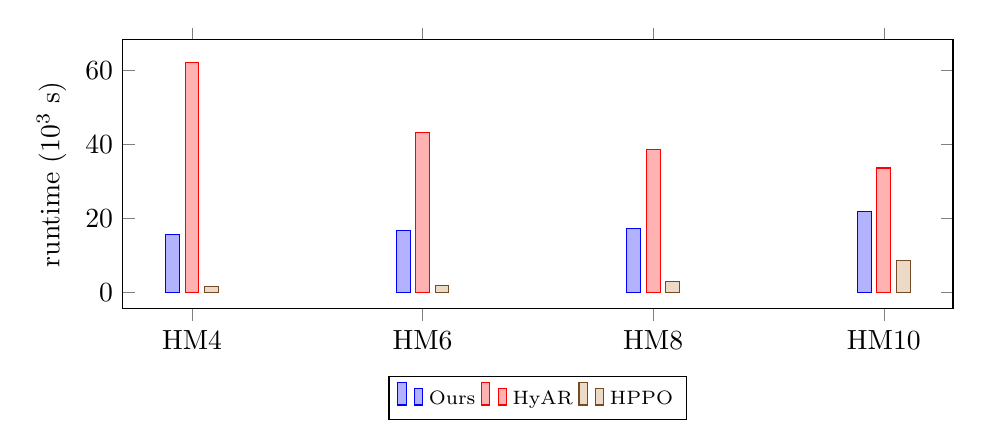
\begin{tikzpicture}\begin{axis}[width=\linewidth,height=5cm,ybar,bar width=5pt,ylabel={runtime (10$^3$ s)},symbolic x coords={HM4,HM6,HM8,HM10},xtick=data,legend style={font=\scriptsize,at={(.5,-.25)},anchor=north,legend columns=3}]
\addplot coordinates {(HM4,15.651)(HM6,16.681)(HM8,17.267)(HM10,21.807)};\addlegendentry{Ours}
\addplot coordinates {(HM4,62.188)(HM6,43.160)(HM8,38.694)(HM10,33.612)};\addlegendentry{HyAR}
\addplot coordinates {(HM4,1.589)(HM6,1.864)(HM8,3.041)(HM10,8.542)};\addlegendentry{HPPO}
\end{axis}\end{tikzpicture}\caption{HardMove measured mean training runtime. HPPO is faster than Ours; HyAR is slower in all four conditions.}\label{fig:hmruntime}\end{figure}
